\documentclass[hidelinks,12pt]{article}
\usepackage[pdftex]{color, graphicx}
\usepackage{amsmath, amsfonts, amssymb, mathrsfs}
%\usepackage{dcolumn}
\usepackage{natbib}
\usepackage{fancyvrb}
\usepackage{hyperref}
%\usepackage{caption}
%\usepackage{subcaption}
%\usepackage{pdfpages}
\usepackage{lscape}
%\usepackage{hangcaption}
\usepackage{multirow}
\usepackage{placeins} % for floatbarrier 
\bibpunct{(}{)}{;}{a}{}{,}

\oddsidemargin=0.25in
\evensidemargin=0.25in
\textwidth=6in
\textheight=9.5in
\topmargin=-1in
\footskip=0.5in

\date{}
\author{Wenyu Gao \& Danni Lu \\ Department of Statistics, Virginia Tech}
\title{STAT 5544 Spatial Analysis Final Project \\ (Fall 2016) \\ Spatial Pattern of Population Movement Using Cellular Data }

\begin{document}
	\maketitle
	
	\begin{abstract}
		As increasing number of people are living in urban area, rising issue such as deteriorating periodical traffic congestion in central business districts is gaining more and more attention. The fundamental question to alleviate traffic congestion in urban area is to figure out where the population origins and how population moves spatially. In this report, we applied a spatiotemporal model to analyze the characteristics of population density in metropolitan based on cellular data. Specifically, taking Shanghai as a case study, the spatial and temporal pattern of population density was discussed. Different spatial models were fitted and compared. Predictions were made based on selected models and the results are displayed in choropleth map. The population movement pattern is discussed based on the map. Results show that during the morning peak hours, population move from all over the city to central areas. Areas with relative high population density expand, grow and converge along transportation corridors. 
	\end{abstract}
	\textbf{ {\em Key words}: Cellular Data, Periodical Traffic, Population Movement, Semivariogram, Spatial Analysis.}
	
	\section{Introduction}\label{sec:intro}
	Recurrent traffic congestion in central business districts is a major sources of cost for transportation system and environments such as pollution. Worldwide, urban population has been growing smoothly during the past decades, from 33.56\% of the world’s population in 1960 to 53.86\% in 2015. In developed country, the proportion is even higher. 82\% of total population in United States was from urban area in 2015(World Bank, 2015). As increasing people are living in urban area, the rising issues such as limited land resource and deteriorating periodical traffic congestion are gaining more and more attention. One of the major causes of periodical traffic congestion is overdevelopment in districts where the traffic attraction exceeds the accommodation volume of traffic system. Central Business Districts (CBD) are therefore becoming controversial as they’re key areas that have been bringing tremendous pressure to transportation system during peak hours in weekday due to their high traffic attraction (Willett K, 2006). 
	
	The CBDs is a major destination for urban area and is major source of traffic demand.  Central Business District (CBD) is the commercial and business center of a city with high developing density. The 21st century CBD within metropolitan areas usually characterized by a concentration of commercial and business buildings, along with other public infrastructure such as entertainment, shopping malls, and medical centers (Olayiwola K O, 2014). According to a traffic survey of 63 cities in US in the 1950s, about one in every five metropolitan residents has at least one destination in the CBD during each weekday (Foley D L, 1952). Integration of multiple services within a small area is of great convenience not only for people living in the vicinity but also for people living elsewhere in the city. However, the price to pay is that area with higher developing density requires transportation system with larger capacity during peak hours in a typical weekday (Mindali O, 2004). Especially in big metropolitan like New York, Sydney and Shanghai. The fact that CBDs are usually geographical center of a city makes the traffic situation even worse. Even though CBDs are facilitated with mass transit system and high capacity road system, the tremendous traffic they attract are usually difficult to accommodate. As a consequence, the traffic congestion in the CBD areas has become a bottleneck for a better city life for every growing metropolitan.
	
	Alleviating periodical traffic congestion is a long term strategy for metropolitan. The very first step should be figuring out the spatial and temporal characteristic of travel behavior during peak hours. This is a classical topic in transportation planning and a lot work has been done since decades ago. Most of the related inferences have been made from traffic survey data. For example, establish models to compute travel time, traffic volume for roads and evaluate optimal routes based on OD survey data (Thériault, 1999).  In early 1950s, Foley and his team collected traffic survey data from municipal officials from more than fifty cities to explore characteristics of travel related to CBD and summarized the quantity and ratio of population who has daily trip destinations in CBD in weekdays (Foley D L, 1954). 
	
	Traditional method to acquire the travel pattern information is conducting household survey, which is usually inefficient and expensive. Nowadays, high density of cellular tower and deep penetration of mobile phones provides us with detailed travel information with high accuracy and precise timing. Some previous study has shown a great potential of mobile data in exploring commuting traffic. As early as 20 years ago, Maryland State Highway Administration conducted a prior project to assess the viability of using cellular-based traffic probes as traffic surveillance technique and demonstrated the technical potential to provide information like travel location, speed and traffic conditions (CAPITAL, 1997). Later, simulation studies were conducted by Virginia Department of Transportation to test the performance of Probe-based traffic monitoring systems. They demonstrated that sampling based on cellular coverage areas is better than other sampling approach in estimating road speed in terms of availability and accuracy (Fontaine, 2007). It’s not until recently that researchers begin to explore travel pattern using real cellular dataset of large scale. Instead of zonal sampling, real cellular dataset has wider coverage and is better representative of population, which allows researchers to study all kinds of travel patterns instead of calculating driving speed of certain road. Cellular data provide us a new way of looking at cities as a dynamic system with detailed information of urban mobility and travel behavior (Reades et al. 2007).  Researchers in Beijing used cellular data to calculate population inflow and outflow volume of selected traffic zone (Dong, Honghui, 2014). Researchers from MIT showed the relationship between home-work travel time and travel distance based on mobile phone call detail records (CDRs). Travel time in Minnesota was also estimated using Cell phone data from Sprint PCS Mobile network (Liu, H. X, 2008). 
	
	Compared with traditional way of exploring travel pattern, cellular data stands out for wider coverage area, better representative of population with all kinds of travel pattern, and more detailed information with high accuracy and precise timing. Thus, cellular data allows us to study temporal and spatial travel characteristics of higher graininess for population in a whole city area. Midtown in Shanghai is one of the largest central business districts in the world, which makes it a perfect study area for travel pattern related to CBD. Based on cellular data collected in Shanghai, we’re going to discuss spatial and temporal characteristics of travel pattern related to CBD in Shanghai. In this study, we treat the study area as a continuous field. First, we established a spatial model to make inference of population density of whole study area. Spatial pattern of population density during each hour in the morning was displayed and the temporal trend of population density was discussed. On the basis, we proposed a method to identify Top Traffic Attraction Zones that attracted most traffic during morning peak hours in a typical weekday. People gathered in Top Traffic Attraction Zones during morning peak are targeted and their trip origins are extracted. At last, we discussed the characteristic of the targeted trips, including the spatial pattern of trip origins, arriving time and distribution of trip distance.
	
	\section{Data Description}\label{sec:data}
	We collected geodetic position information of all users in Shanghai from China Mobile for a continuous 24-hour period. China Mobile is the biggest carrier in China, with 64\% total ownership in China (China Mobile, China Unicom and China Telecom, 2016). The dataset includes coded mobile phone ID, date, time, latitude and longitude of corresponding cellular tower. Cellular towers are infrastructure that enables voice and data services for mobile phones. They operate in different radio frequencies, and allow users to maintain their connections while traveling from one base station to another. In total, we collected more than 1.1 billion cell tower hands-off records. These records are from 37,450 different cell towers all over Shanghai with average density of 5.91 cell tower per kilometer square.
	
	One issue of adopting cellular data is privacy of participants (Steenbruggen, John, 2013). To protect their privacy, all records are anonymized and replaced by an identifier ID before we got access to it. In addition, records were aggregated by areal unit and time period before analyzing and visualizing. No personal information is involved and displayed in the research.
	
	The spatial pattern of population density has a direct relationship with traffic demand.  Every morning on weekday, metropolitan sees a population movement from every corner of the city to CBD areas. During peak hours, the traffic on roads and crowding transport is at its highest. The huge increment of population brings tremendous pressure to transportation system near CBD areas. In traditional traffic survey, no standard areal definition of CBD was followed (Foley D L., 1952). Though the importance of CBD in transportation is self-evident, it is much more of a general concept in transportation study. Luckily, the comprehensive information of cellular data provides us a way to identify CBD by its transportation characteristics. In this study, we focus on main districts that are circled by Outer Expressway in Shanghai (Figure \ref{fig:area}).
	\begin{figure}[!ht]
		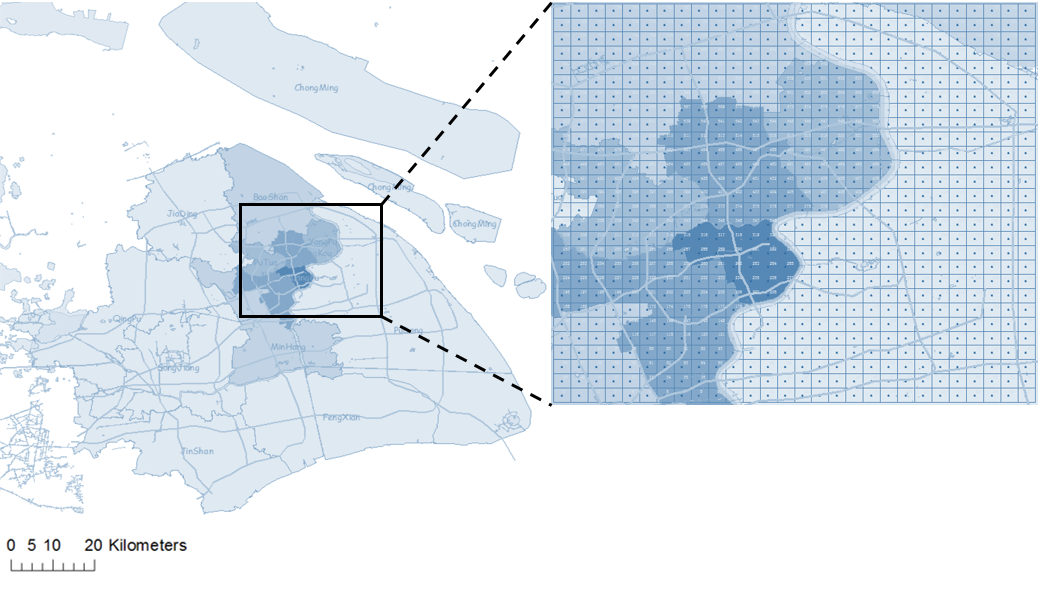
\includegraphics[width=\textwidth]{area.png}
		\caption{Study Area and Aggregation Grid \label{fig:area}}
	\end{figure}
	The accuracy of location information we get depends on the density of cell towers. Instead of accurate location of mobile phone users, cellular data recorded location of cell tower that is nearest to the mobile phone users. As we can see in Figure \ref{fig:tower}, cell towers are not evenly spaced. The density in the center area is higher than outer areas. As a result, the coverage area of each cellular tower is different. To simplify the situation, study area is partitioned into a 28*28 grid, each areal unit is one square kilometer. All cellular information from one areal unit is aggregated into one fictional cell tower in the geo-center of the areal unit (Figure \ref{fig:tower}). Hence, we have a regular point-referenced data to establish spatial model. In terms of study period, our goal is exploring spatial and temporal pattern of population in rush hours in the morning. Previous study shows typical morning rush hours for metropolitan CBDs are between 7:00 and 9:00 am. Therefore, we extract cellular data from 5:00 am to 10:00 am to cover this range.
	\begin{figure}[!ht]
		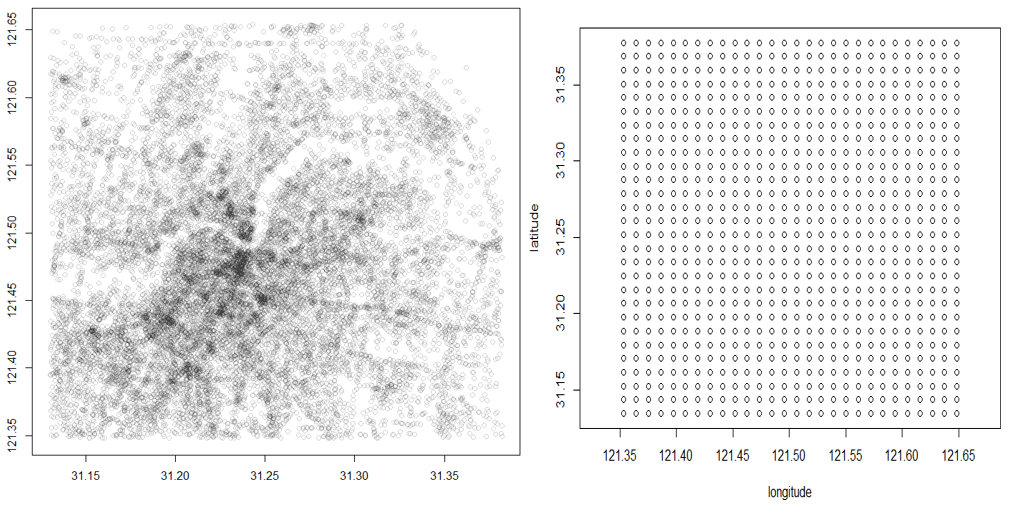
\includegraphics[width=\textwidth]{tower.png}
		\caption{Original Cell Towers and Aggregated Cell Towers \label{fig:tower}}
	\end{figure}
	
	\section{Methodologies}\label{sec:meth}
	Based on our data characteristics and aggregation methods, we treat our data as point-referenced data and apply the corresponding spatial theories for analysis. The whole analyzing process is as follows: We begin from exploratory analysis to check if there is any special structure of the data. Then followed by identification of spatial trend. We would like to analyze the data without spatial trends because this will reflect the intrinsic covariance structure of the data. After detrending, we will check for existence of anisotropy. Model fitting will be conducted after all these preliminary work has been done. Semivariogram fitting and likelihood fitting models are considered. Some model selection criteria are applied to select the best fit and predicted model. Last but not least, we will make inference on the predicted models.
	
	Most of the preliminary checks are based on visualization, except for spatial trend detection, where model fitting is conducted. The trend is mainly diagnosed with coordinates.
	
	\section{Results}\label{sec:res}
	\subsection{Exploratory Data Analysis}\label{sec:reseda}
	We begin with a summary table of the dataset, shown in Table \ref{tbl:sumdata}.
	% latex table generated in R 3.3.1 by xtable 1.8-2 package
	% Mon Dec 05 20:09:50 2016
	\begin{table}[ht]
		\centering
		\caption{Summary Table of Dataset \label{tbl:sumdata}}
		\begin{tabular}{rllll}
			\hline
			&      FID &      long &      lat &      freq  \\ 
			\hline
			1 & Min.   :  0.0   & Min.   :121.4   & Min.   :31.13   & Min.   :    0     \\ 
			2 & 1st Qu.:195.8   & 1st Qu.:121.4   & 1st Qu.:31.20   & 1st Qu.: 2060     \\ 
			3 & Median :391.5   & Median :121.5   & Median :31.26   & Median : 5894    \\ 
			4 & Mean   :391.5   & Mean   :121.5   & Mean   :31.26   & Mean   : 9773      \\ 
			5 & 3rd Qu.:587.2   & 3rd Qu.:121.6   & 3rd Qu.:31.32   & 3rd Qu.:14575    \\ 
			6 & Max.   :783.0   & Max.   :121.6   & Max.   :31.38   & Max.   :83822      \\ 
			\hline
			 &    D2Metro &     D2Road &      hour &\\
			\hline
			1  & Min.   :   0.395 & Min.   :   2.274   & Min.   :5 &\\
			2    & 1st Qu.: 387.974  & 1st Qu.: 397.764   & 1st Qu.:6 & \\
			3   & Median : 973.144  & Median : 888.332   & Median :7 &\\
			4  & Mean   :1373.922 & Mean   :1126.451   & Mean   :7 &\\
			5   & 3rd Qu.:1981.959 & 3rd Qu.:1609.672   & 3rd Qu.:8  &\\
			6   & Max.   :6852.305 & Max.   :5607.713   & Max.   :9 & \\
			\hline
		\end{tabular}
	\end{table}
	From the table, it is clear to see that the locations do not vary greatly in longitude and latitude. The frequency, distance to Metro and distance to road have large range and do not seem to be symmetric. There seems no problematic data. We then focus on the frequency variable and we will check the image plot (Figure \ref{fig:image}), perspective plot (Figure \ref{fig:perp} in Appendix \ref{sec:appa}), histogram (Figure \ref{fig:hist}), boxplot (Figure \ref{fig:boxplot} in Appendix \ref{sec:appa}) and qqplot (Figure \ref{fig:qq} in Appendix \ref{sec:appa}) on the variable. Due to page limitation, we only present the image plot and histograms in the paper. The other plots are put to appendices.
	\begin{figure}[!ht]
		\includegraphics[width=\textwidth]{image.png}
		\caption{Image Plots of Frequency by Hour \label{fig:image}}
	\end{figure}
	\FloatBarrier
	\begin{figure}[!ht]
		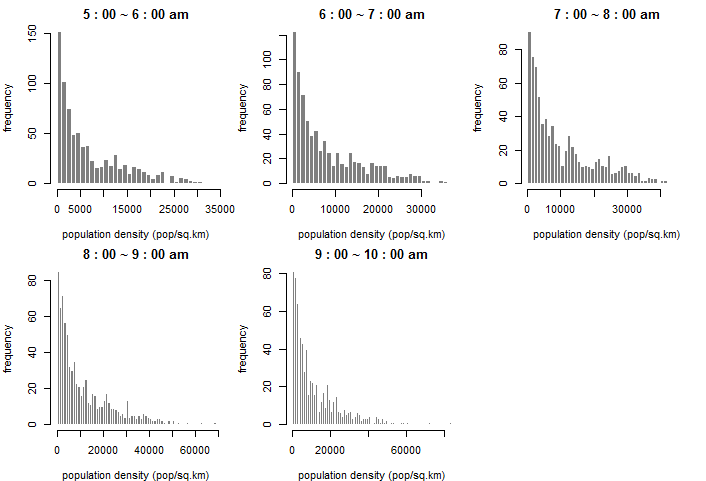
\includegraphics[width=\textwidth]{hist.png}
		\caption{Histograms of Frequency by Hour \label{fig:hist}}
	\end{figure}
	\FloatBarrier
	\begin{figure}[!ht]
		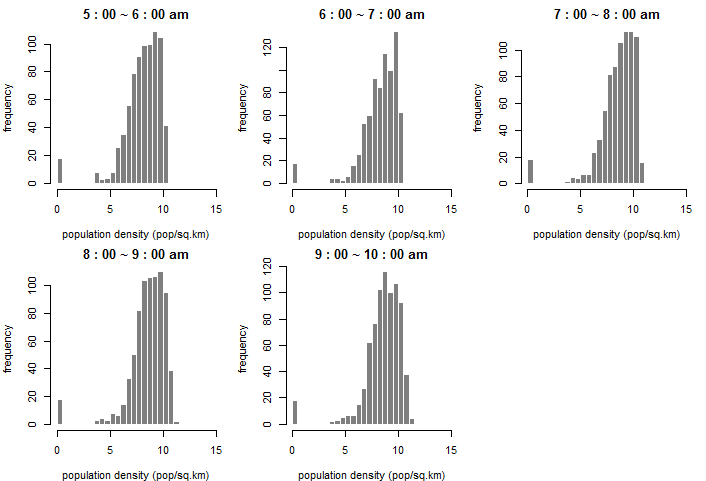
\includegraphics[width=\textwidth]{hist_log.png}
		\caption{Histograms of log-Frequency by Hour \label{fig:lghist}}
	\end{figure}
\FloatBarrier

	Image plots are set to be the same scales where dark red color represents low values while bright yellow colors indicate high values. It is clear that bright colors are centered in the middle and the color becomes brighter and brighter by time. That is, more people are gathering to CBD by time.
	
	Histograms show that frequency is highly skewed. However, after log transformation, the histograms are still not desirable (shown in Figure \ref{fig:lghist}). Similarly, boxplot and qqplot also show that variable frequency does not follow normal distribution. After log transformation, it is still not normally distributed.

\subsection{Spatial Trend}\label{sec:spatialtrend}

In order to prepare spatial data for stationarity procss analysis, we need to check the correlation between the response and location. Side by side bar plot is used to demonstrate the relationship between response and location. Population density with respect to latitude and longitude is shown in Figure \ref{fig:lat} and Figure \ref{fig:long} respectively. As is shown, there is a curvature relationship between population density and two coordination variables. 

\begin{figure}[!ht]
		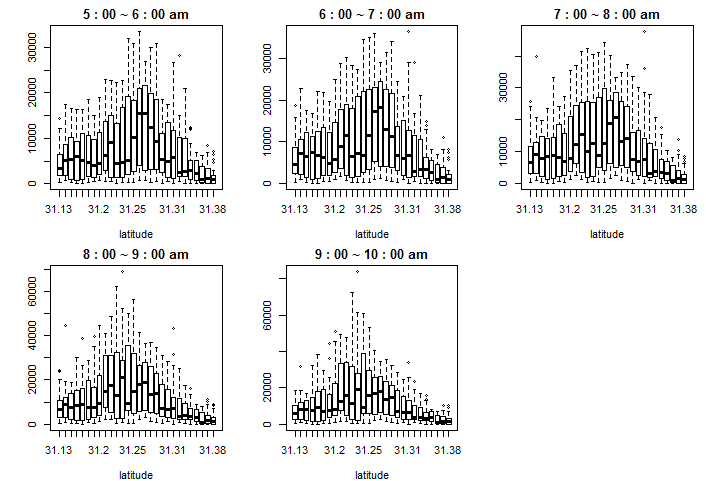
\includegraphics[width=\textwidth]{lat.png}
		\caption{Population Density and Latitude\label{fig:lat}}
\end{figure}
\FloatBarrier

\begin{figure}[!ht]
		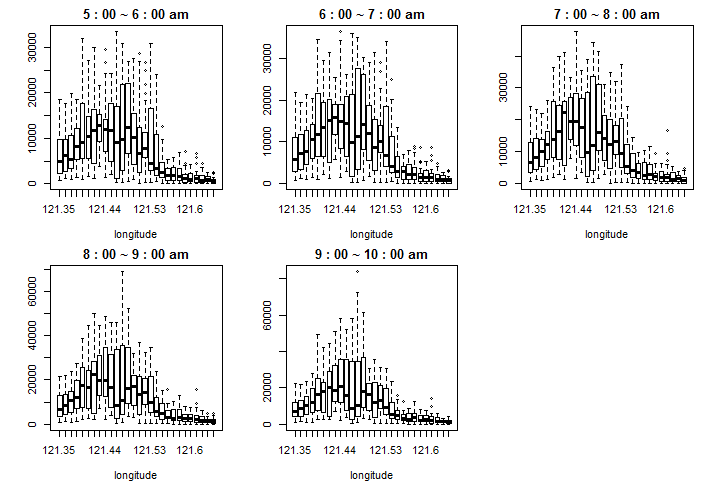
\includegraphics[width=\textwidth]{long.png}
		\caption{Population Density and Longitude\label{fig:long}}
\end{figure}
\FloatBarrier

Therefore, we fit polynomial regression of order two to remove the underlying spatial trend. Naturally, we set population density as response. Covariates include latitude, longitude, their quadratic term and interaction. Stepwise selection is used for variable screening. Under AIC criterion, full model (Model \ref{mod:polyreg} ) is selected for its best performance.

\begin{align}
\label{mod:polyreg}
Y(s_i)=\beta_0 +\beta_1x_{1i} +\beta_2x_{2i} +\beta_3x_{1i}^2 +\beta_4x_{2i}^2+\beta_5x_{1i}x_{2i}+\epsilon_i
\end{align}
where,
$Y(s_i)$ is population density at location $s_i$;\\
$x_{1i}$ is latitude of location $s_i$;\\
$x_{2i}$ is longitude of location $s_i$;\\
and corresponding estimates are:\\
$\hat{\beta_0}=-4.524*10^9$;\\
$\hat{\beta_1}=2.018*10^7$;\\
$\hat{\beta_2}=6.932*10^7$;\\
$\hat{\beta_3}=-5.698*10^5$;\\
$\hat{\beta_4}=-3.018*10^5$;\\
$\hat{\beta_5}=1.271*10^5$.\\

Thus,instead of using population density, residuals for each location produced in Model \ref{mod:polyreg} are used to conduct spatial analysis in the following sections.

\subsection{Anisotropy}\label{sec:anis}
Isotropy means the covariance function of the spatial random variable depends on the displacement vector only through its length. This is always a desirable property as it simplifies the covariance structure and we can express the covariance structure as a function of distance. \\

To check for isotropy assumption, two widely used methods are to look at the empirical semivariogram contour plots and directional semivariance plots. First we start with directional semivariance plot shown in Figure \ref{fig:dir_semi}. The plots show that semivariances for different direction are close to each other except the tail part where sample size is small, indicating there is no significant difference in semivariance among all the direction plotted. For complementary, we further check the empirical semivariogram contour plots shown in Figure \ref{fig:esc}. The contour plot shows unique peak in the center of study area, outlined by circular contour lines which indicating an acceptable isotropy situation.

\begin{figure}[!ht]
		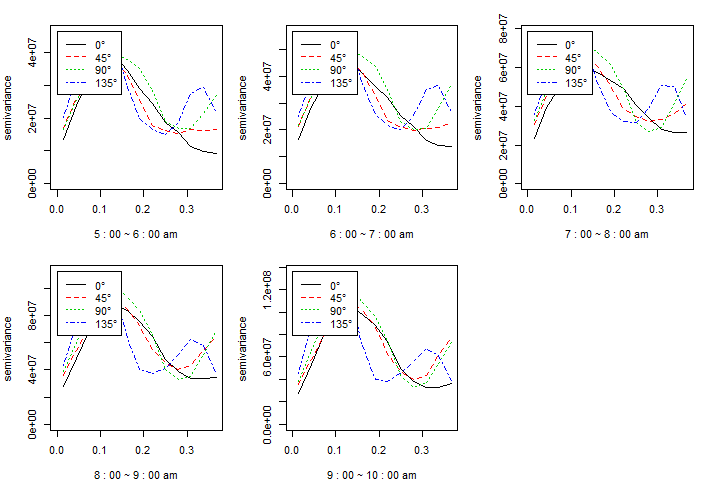
\includegraphics[width=\textwidth]{dir_semi.png}
		\caption{Directional Semivariance Plots\label{fig:dir_semi}}
\end{figure}
\FloatBarrier

\begin{figure}[!ht]
		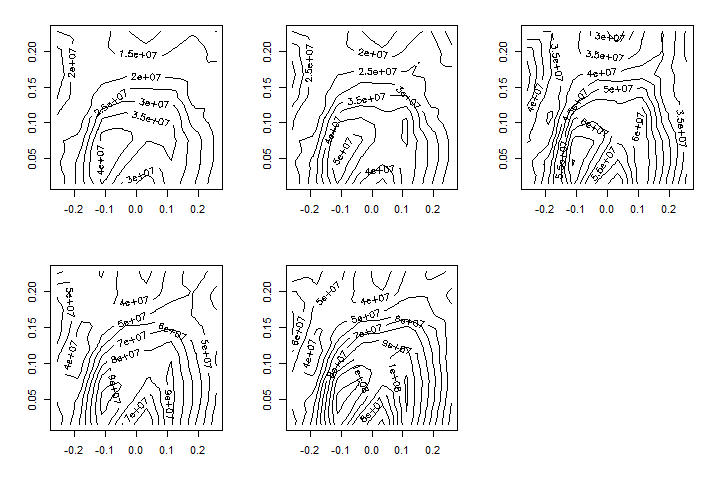
\includegraphics[width=\textwidth]{esc.png}
		\caption{Empirical Semivariogram Contour plot\label{fig:esc}}
\end{figure}
\FloatBarrier




	\section{Conclusion}\label{sec:con}
	
	\section{Reference}\label{sec:ref}
	\bibliography{sample}
	
	\newpage
	\appendix
	\section{Appendices -- Plots} \label{sec:appa}
	\begin{figure}[!ht]
		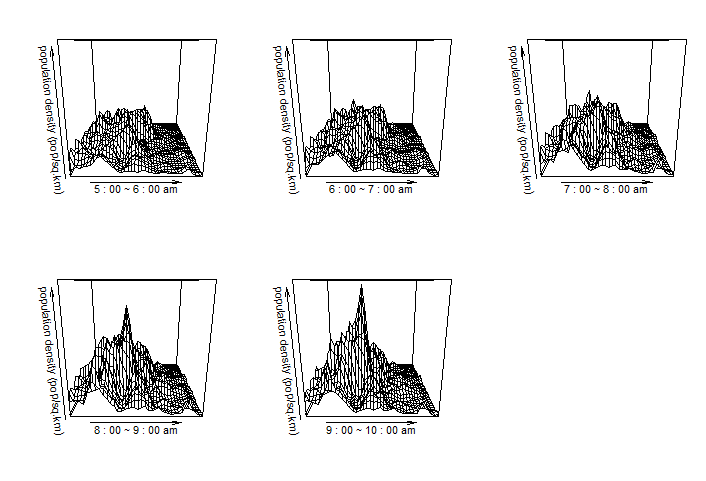
\includegraphics[width=\textwidth]{persp.png}
		\caption{Perspective Plot of Frequency by Hour \label{fig:perp}}
	\end{figure}
	\begin{figure}[!ht]
		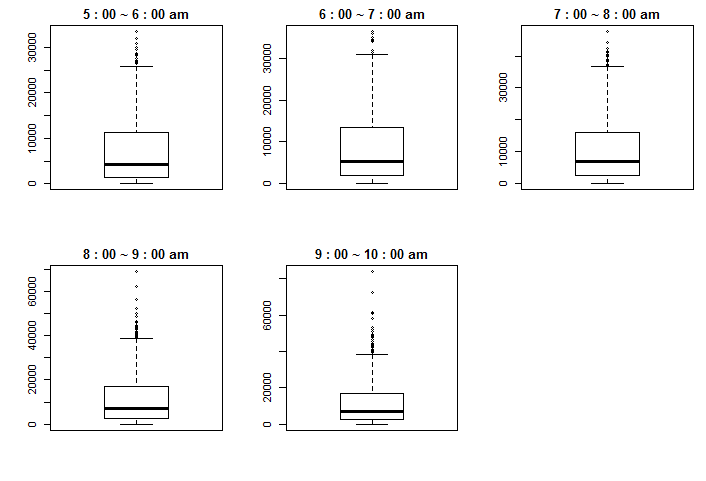
\includegraphics[width=\textwidth]{box.png}
		\caption{Boxplots of Frequency by Hour \label{fig:boxplot}}
	\end{figure}
	\begin{figure}[!ht]
		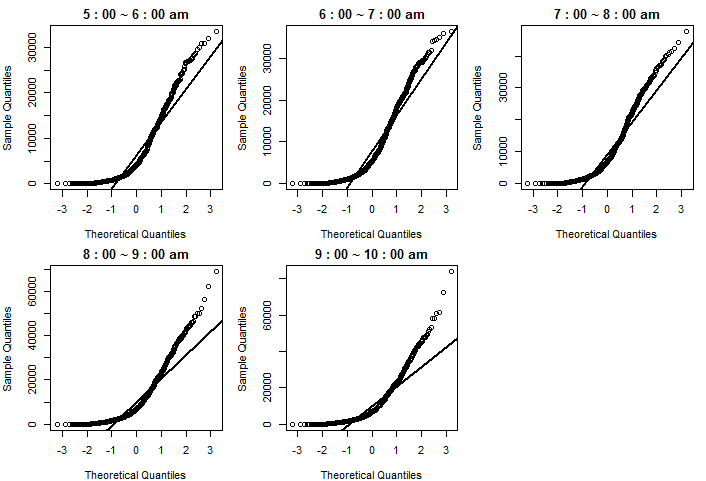
\includegraphics[width=\textwidth]{qq.png}
		\caption{QQ-Plots of Frequency by Hour \label{fig:qq}}
	\end{figure}
	\begin{figure}[!ht]
		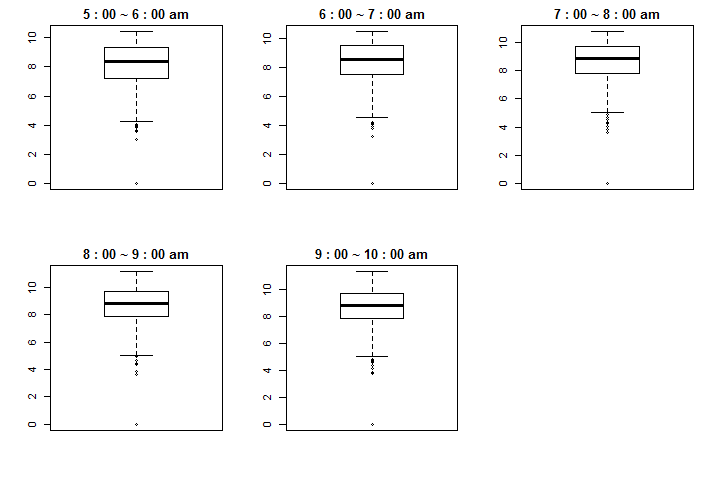
\includegraphics[width=\textwidth]{box_log.png}
		\caption{Boxplots of log-Frequency by Hour \label{fig:lgboxplot}}
	\end{figure}
	\begin{figure}[!ht]
		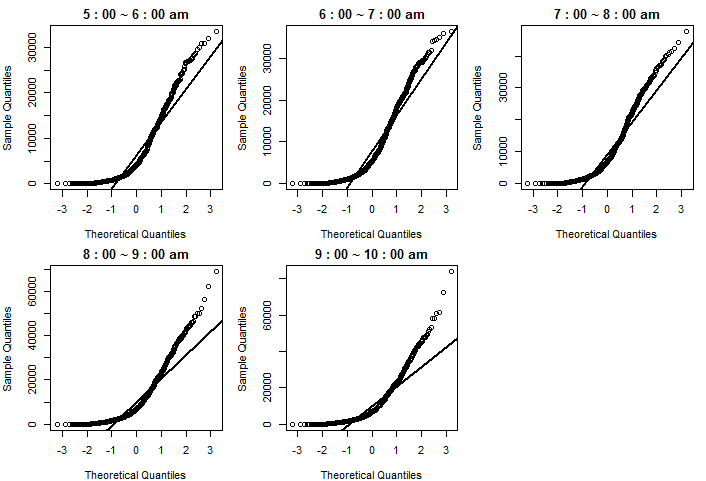
\includegraphics[width=\textwidth]{qq.png}
		\caption{QQ-Plots of log-Frequency by Hour \label{fig:lgqq}}
	\end{figure}

	\section{Appendices -- R codes}
	\begin{verbatim}
		
	\end{verbatim}
	
\end{document}